\documentclass{article}
\usepackage{enumitem}
\usepackage{listings}
\usepackage{amsfonts}
\usepackage{latexsym}
\usepackage{fullpage}
\usepackage{graphicx}
\usepackage{paralist}
\usepackage{tikz-timing}

\lstdefinelanguage{VHDL}{
  morekeywords={
    library,use,all,ENTITY,IS,PORT,IN,OUT,end,architecture,of,
    begin,and, ARCHITECTURE, IF, THEN, SIGNAL,END, PROCESS
  },
  morecomment=[l]--
}

\usepackage{xcolor}
\colorlet{keyword}{blue!100!black!80}
\colorlet{comment}{green!90!black!90}
\lstdefinestyle{vhdl}{
  language     = VHDL,
  basicstyle   = \ttfamily\scriptsize,
  keywordstyle = \color{keyword}\bfseries\ttfamily,
  commentstyle = \color{comment}\ttfamily,	
  tabsize=1
}

\renewcommand{\lstlistingname}{Code}

% Default margins are too wide all the way around. I reset them here
\setlength{\topmargin}{-.5in}
\setlength{\textheight}{9in}
\setlength{\oddsidemargin}{.125in}
\setlength{\textwidth}{6.25in}


%\let\oldenumerate\enumerate
%\renewcommand{\enumerate}{
  %\oldenumerate
  %\setlength{\itemsep}{1pt}
  %\setlength{\parskip}{0pt}
  %\setlength{\parsep}{0pt}
%}


\begin{document}
\title{Single-Cycle MIPS Processor}
\author{prepared by: David Pynes and Andrew Sperry \\ \\  
{February, 13, 2016}}


\date{}
\maketitle


\section{Synopsis}
 
	\subsection{Description}
		This project consisted of completing the single-cycle MIPS processor. Hexadecimal format instructions are preloaded from an external file, converted to 32-bit binary, and loaded into the ROM at the start of the simulation. The processor has been expanded to support the following instructions: \textbf{add, sub, addi, addu, subu, addiu, and, andi, or, ori, nor, xor, xori, andi, ori, xori, sll, srl, sra, sllv, srlv, srav, slt, sltu, slti, sltiu, jump, jal, jr, jalr, beq, bne, bltz, bgez, blez, bgtz, lui, lb, lbu, lh, lhu, lw, sb, sh, and sw}. In future projects, the component design will be converted to a pipe-lined model.\\ \\ 
	This project has been coded in VHDL using the ISE Xlinix environment. Verilog was used for component and processor test-benches and xxx was used for synthesizing and optimization. Within the processor, test ports were added to ensure components were operating correctly at each stage of the datapath design and testing phases. Various bugs were found mostly in controller logic when testing each of the above instructions.  \\ \\
	To support the new design, read-only memory and random-access memory were both converted to a byte addressable design. Byte, half-word and word load logic were placed inside of the random-access memory to optimize the design. This change required an additional type bit be connected to random-access memory but also eliminated the need for the 2-bit load control needed in the previous design. \\ \\
	\section{Datapath:}
	
	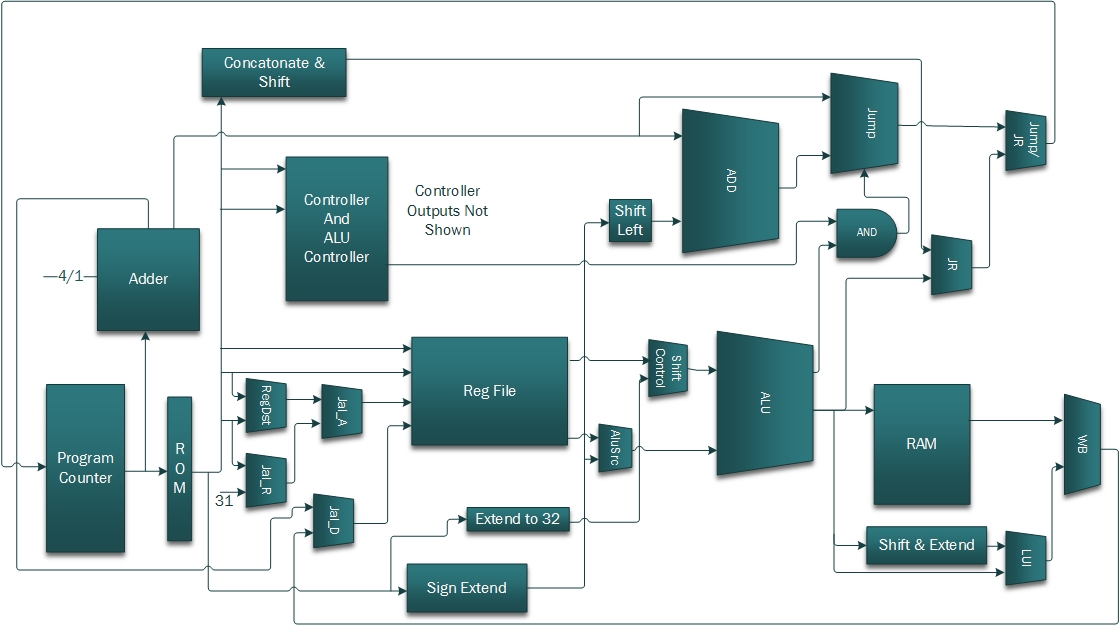
\includegraphics[width=1\columnwidth]{datapath.jpg} \\ \\
	
		The figure above does not shown controller output signals connected to the following components: \textbf{RegDis\_Control, Jal\_R\_Control, Jal\_D\_Control, Jal\_A\_Control, RegWrite, ALUSrc, ShiftValue, ALUOpcode, JR\_Control, JumpOrJr\_Control, DSize, VType, LUI\_Control, and WB\_Control}.

	\section{Test Program Waveforms:}
	I1 -- 20020005 \\
	I2 -- 2003000c \\
	I3 -- 2067fff7 \\
  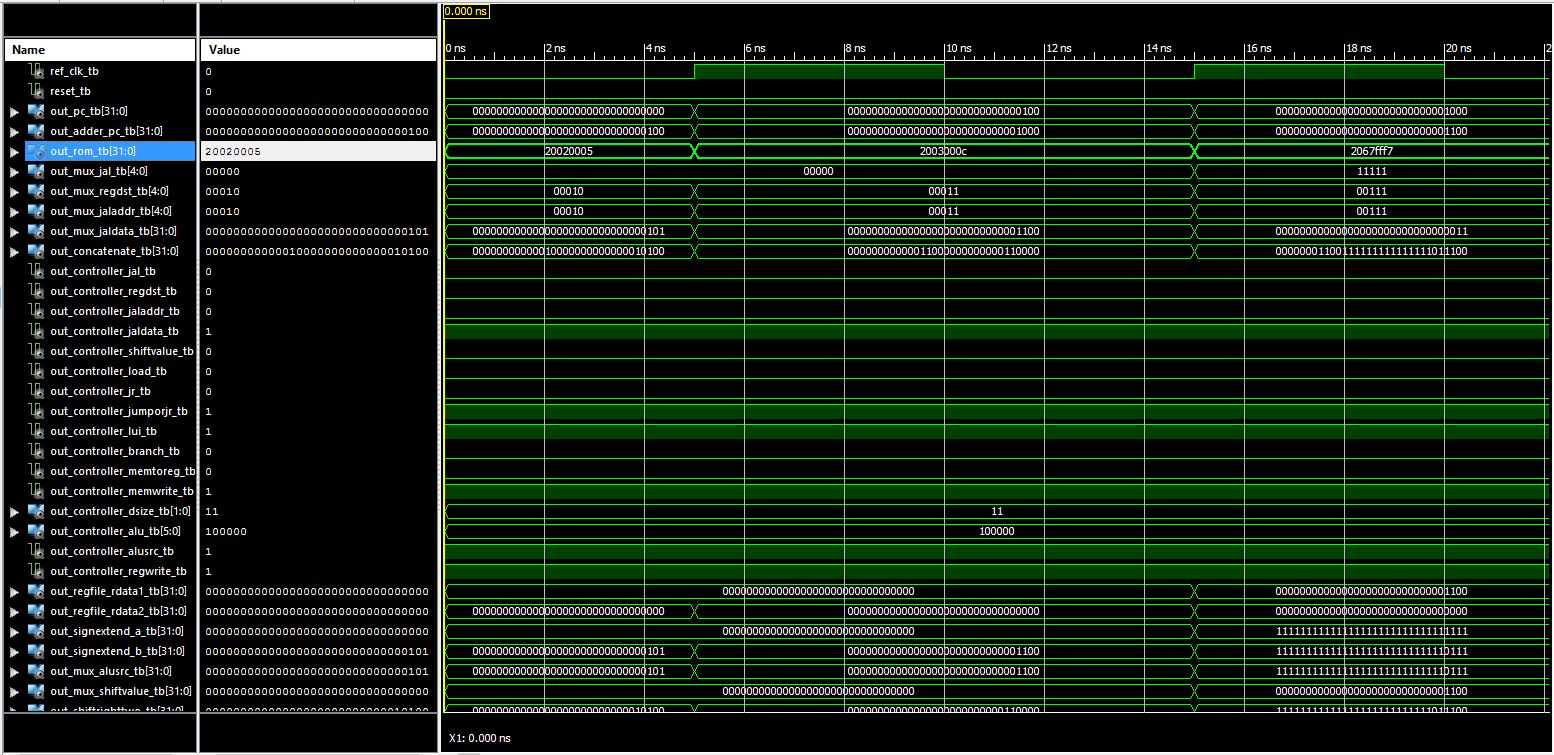
\includegraphics[width=1\columnwidth]{i01.JPG}
	\\
	I4 -- 00e22025 \\
	I5 -- 00642824 \\
	I6 -- 00a42820 \\
  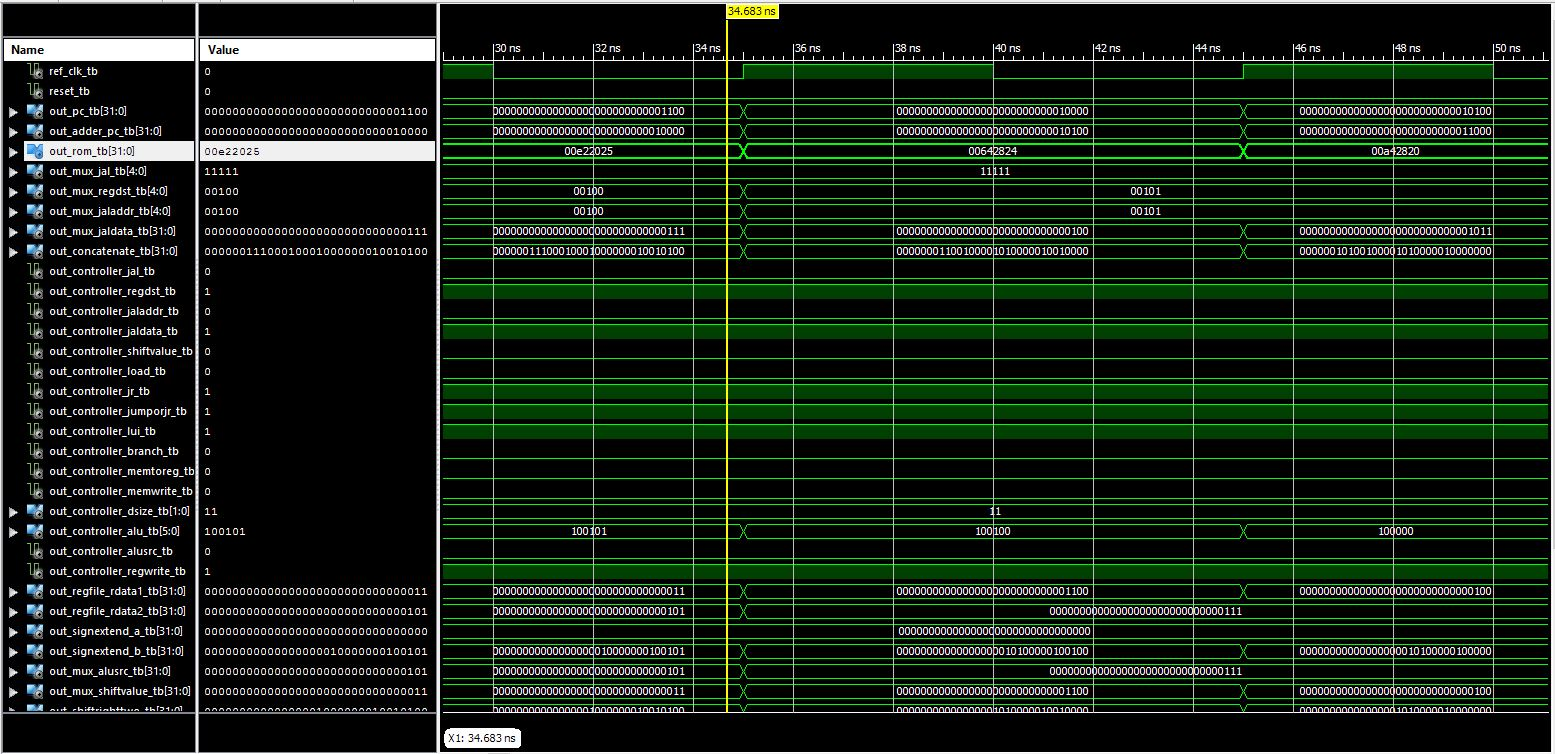
\includegraphics[width=1\columnwidth]{i02.JPG}
	\\
	I7 -- 10a7000a \\
	I8 -- 0064202a \\
	I9 -- 10800001 \\
  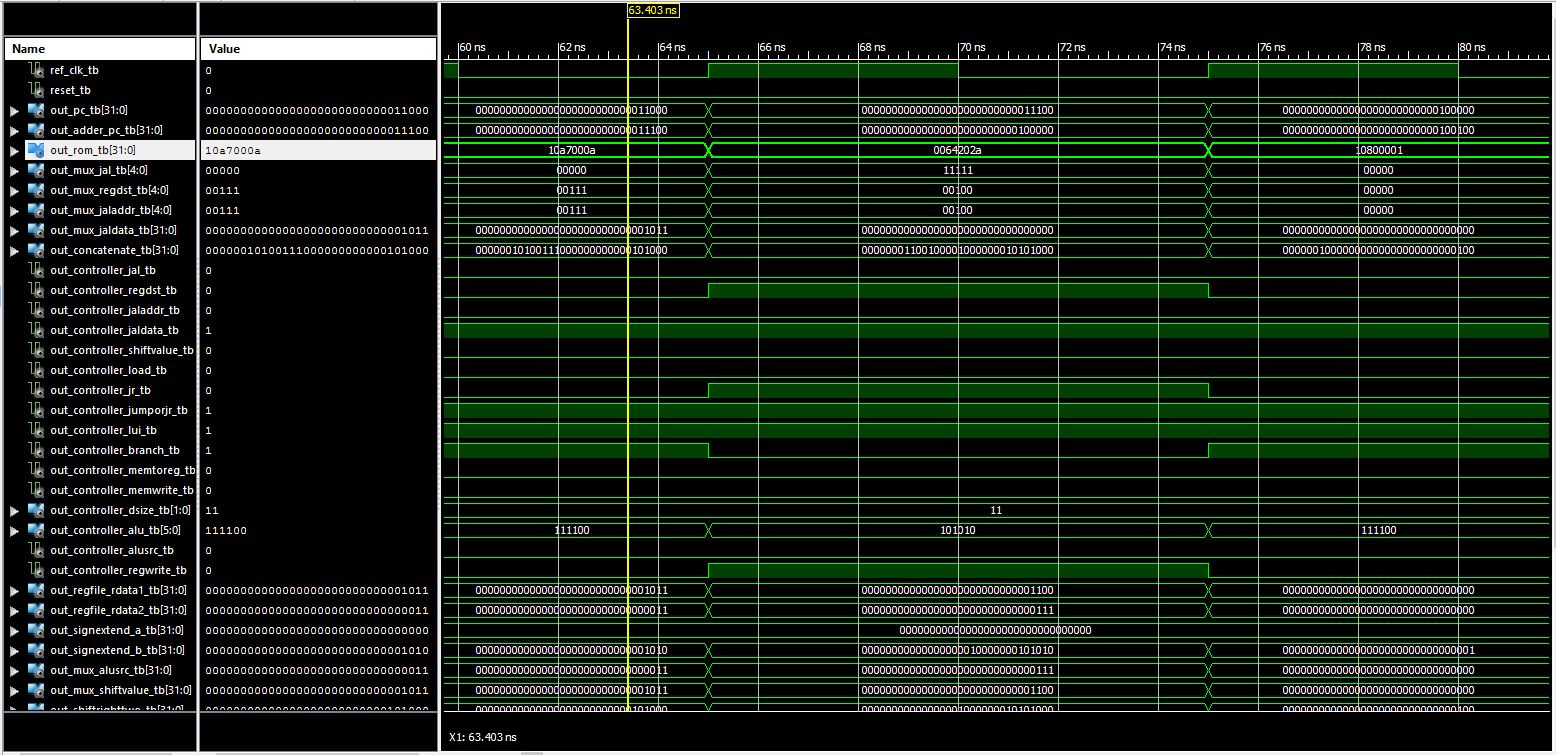
\includegraphics[width=1\columnwidth]{i03.JPG}
	\\
	I10 -- 20050000 \\
	I11 -- 00e2202a \\
	I12 -- 00853820 \\
  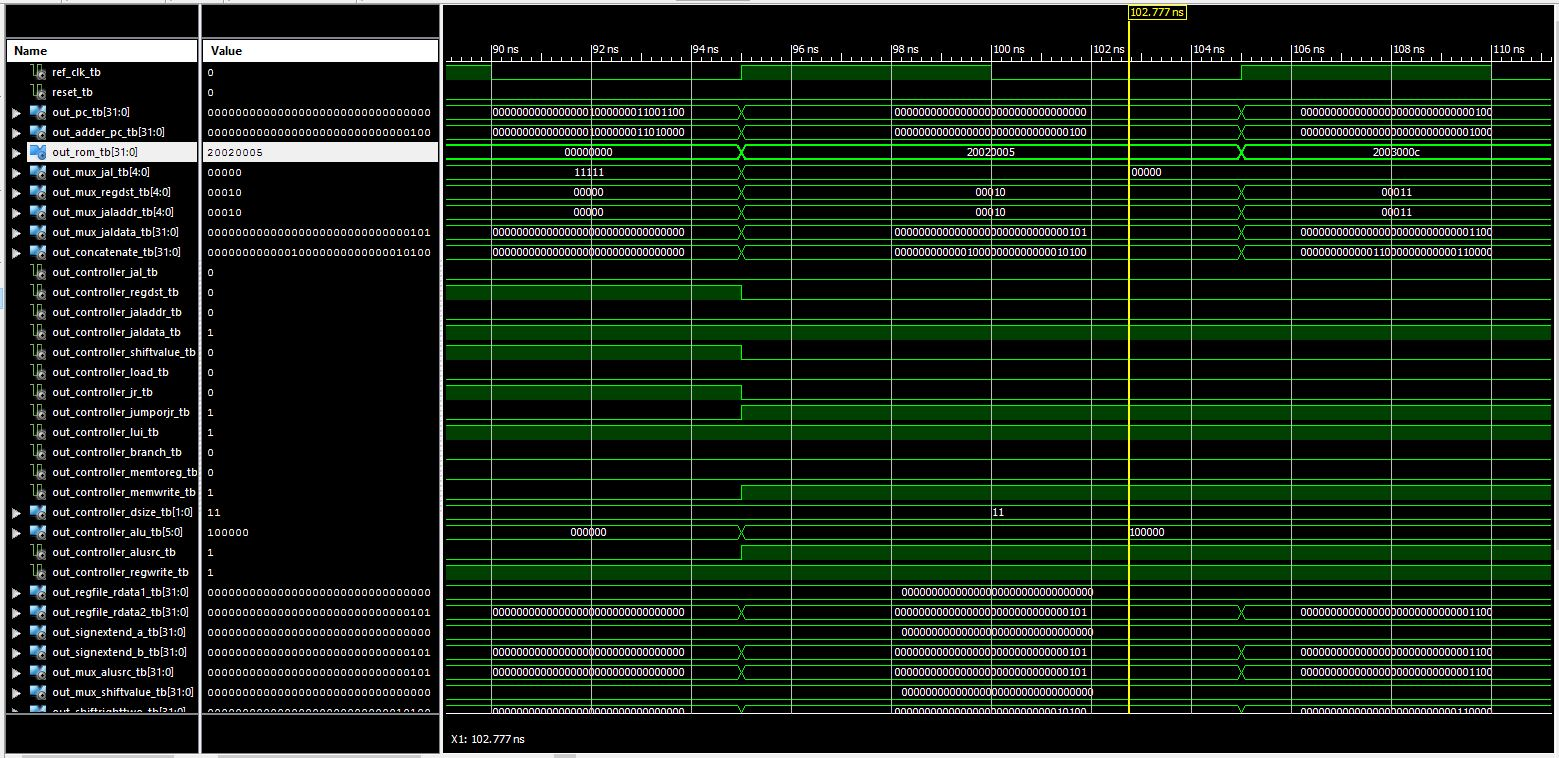
\includegraphics[width=1\columnwidth]{i04.JPG}
	\\
	I13 -- 00e23822 \\
	I14 -- ac670044 \\
	I15 -- 8c020050 \\
  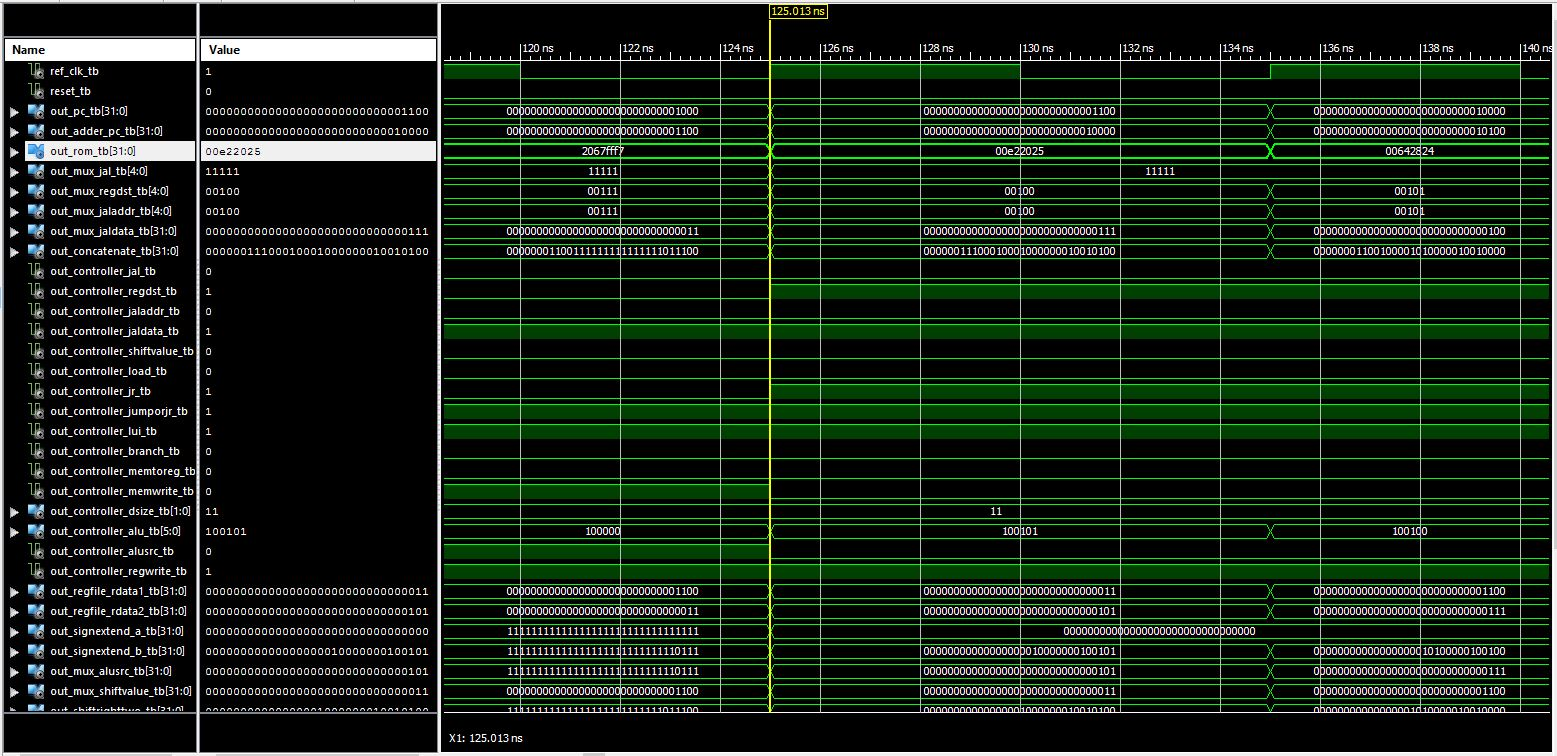
\includegraphics[width=1\columnwidth]{i05.JPG}
	\\
	I16 -- 08000011 \\
	I17 -- 20020001 \\
	I18 -- ac020054 \\
  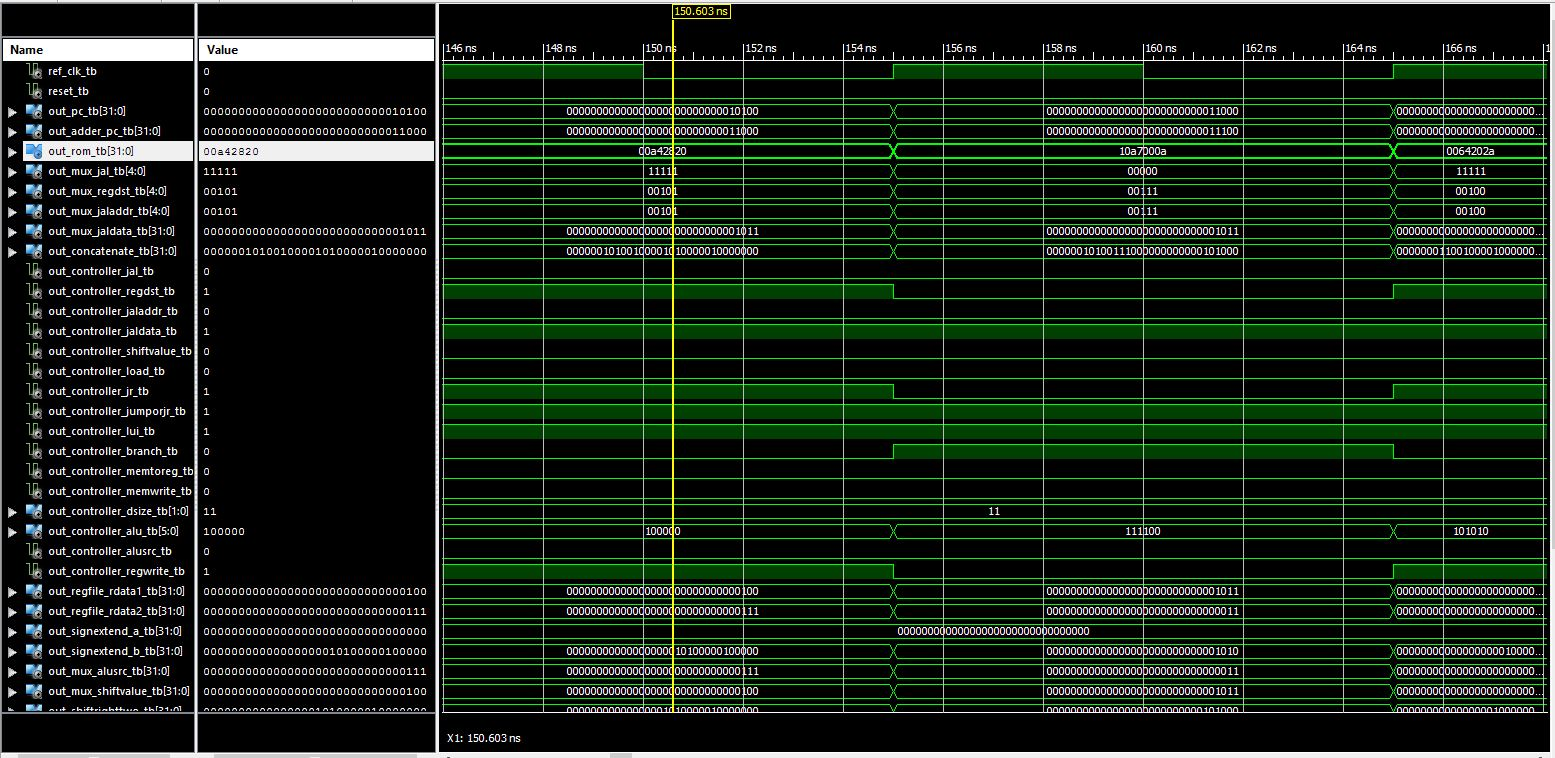
\includegraphics[width=1\columnwidth]{i06.JPG}
	
\section{Sample Program}

	We were able to successfully decode what each of the sample programs instructions did and verified one-by-one that they operated correctly as shown in the waveform images above.\\ \\
	
\section{Problem Areas}

	During the development of this processor, most of our logical errors occurred when developing the controller component. It was a lengthy process to map the path and controller settings needed for each required instruction. Often times, the first test of each instruction resulted in controller outputs not being set correctly, leading to further analysis of the circuit image to hunt down and fix logical errors.\\ \\
	Opposite of logical errors, most of our syntax errors took place in the processor and processor tesh\-bench files. With the need to make so many connections between components as well as the added use of several test-only ports, there was a lot of code that could easily get typed incorrectly.\\ \\
	In the end, we were able to resolve all logical and syntax errors which allowed our processor to operate in a stable and accurate manner.

\section{Synthesis Report}
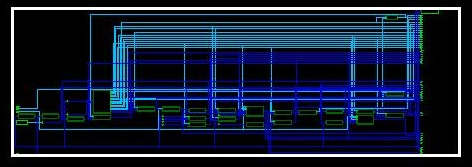
\includegraphics[width=1\columnwidth]{RTLSchematic.JPG}
	After successful synthesizing and optimization of our processor, the following results were obtained by the synthesis report: \\
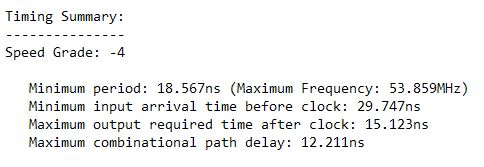
\includegraphics[width=1\columnwidth]{SynthesisReport.JPG}


\end{document}
